\documentclass[]{article}
\usepackage{lmodern}
\usepackage{amssymb,amsmath}
\usepackage{ifxetex,ifluatex}
\usepackage{fixltx2e} % provides \textsubscript
\ifnum 0\ifxetex 1\fi\ifluatex 1\fi=0 % if pdftex
  \usepackage[T1]{fontenc}
  \usepackage[utf8]{inputenc}
\else % if luatex or xelatex
  \ifxetex
    \usepackage{mathspec}
  \else
    \usepackage{fontspec}
  \fi
  \defaultfontfeatures{Ligatures=TeX,Scale=MatchLowercase}
\fi
% use upquote if available, for straight quotes in verbatim environments
\IfFileExists{upquote.sty}{\usepackage{upquote}}{}
% use microtype if available
\IfFileExists{microtype.sty}{%
\usepackage{microtype}
\UseMicrotypeSet[protrusion]{basicmath} % disable protrusion for tt fonts
}{}
\usepackage[margin=1in]{geometry}
\usepackage{hyperref}
\hypersetup{unicode=true,
            pdftitle={Presentation of Ancestral Reconstruction Results},
            pdfauthor={J.P. Meagher},
            pdfborder={0 0 0},
            breaklinks=true}
\urlstyle{same}  % don't use monospace font for urls
\usepackage{graphicx,grffile}
\makeatletter
\def\maxwidth{\ifdim\Gin@nat@width>\linewidth\linewidth\else\Gin@nat@width\fi}
\def\maxheight{\ifdim\Gin@nat@height>\textheight\textheight\else\Gin@nat@height\fi}
\makeatother
% Scale images if necessary, so that they will not overflow the page
% margins by default, and it is still possible to overwrite the defaults
% using explicit options in \includegraphics[width, height, ...]{}
\setkeys{Gin}{width=\maxwidth,height=\maxheight,keepaspectratio}
\IfFileExists{parskip.sty}{%
\usepackage{parskip}
}{% else
\setlength{\parindent}{0pt}
\setlength{\parskip}{6pt plus 2pt minus 1pt}
}
\setlength{\emergencystretch}{3em}  % prevent overfull lines
\providecommand{\tightlist}{%
  \setlength{\itemsep}{0pt}\setlength{\parskip}{0pt}}
\setcounter{secnumdepth}{0}
% Redefines (sub)paragraphs to behave more like sections
\ifx\paragraph\undefined\else
\let\oldparagraph\paragraph
\renewcommand{\paragraph}[1]{\oldparagraph{#1}\mbox{}}
\fi
\ifx\subparagraph\undefined\else
\let\oldsubparagraph\subparagraph
\renewcommand{\subparagraph}[1]{\oldsubparagraph{#1}\mbox{}}
\fi

%%% Use protect on footnotes to avoid problems with footnotes in titles
\let\rmarkdownfootnote\footnote%
\def\footnote{\protect\rmarkdownfootnote}

%%% Change title format to be more compact
\usepackage{titling}

% Create subtitle command for use in maketitle
\newcommand{\subtitle}[1]{
  \posttitle{
    \begin{center}\large#1\end{center}
    }
}

\setlength{\droptitle}{-2em}
  \title{Presentation of Ancestral Reconstruction Results}
  \pretitle{\vspace{\droptitle}\centering\huge}
  \posttitle{\par}
  \author{J.P. Meagher}
  \preauthor{\centering\large\emph}
  \postauthor{\par}
  \predate{\centering\large\emph}
  \postdate{\par}
  \date{\today}

\usepackage{tikz}
\usepackage{float}

\begin{document}
\maketitle

\section{Introduction}\label{introduction}

We are given a dataset of \(N\) bat echolocation call recordings denoted \(\{y_n\}_{n = 1}^N\). This recording is then processed to produce a set of smooth surfaces over a regular grid denoted \(\{\tilde{S}_n\}_{n=1}^{N}\). This surface, referred to as the call surface hereafter, is produced by smoothing the call spectrogram and mapping it to a regular grid over relevant frequencies and an absolute time scale in the manner as outlined by Pigoli \textit{et al.} \cite{pigoli2015analysis}. A robust N-D spline smoothing algorithm presented by Garcia \cite{garcia2010robust} was implemented for surface smoothing and a pairwise curve synchronisation algorithm by Tang \& Muller \cite{tang2008pairwise} was extended to surfaces for time registration.

\begin{figure}[htbp]
\centering
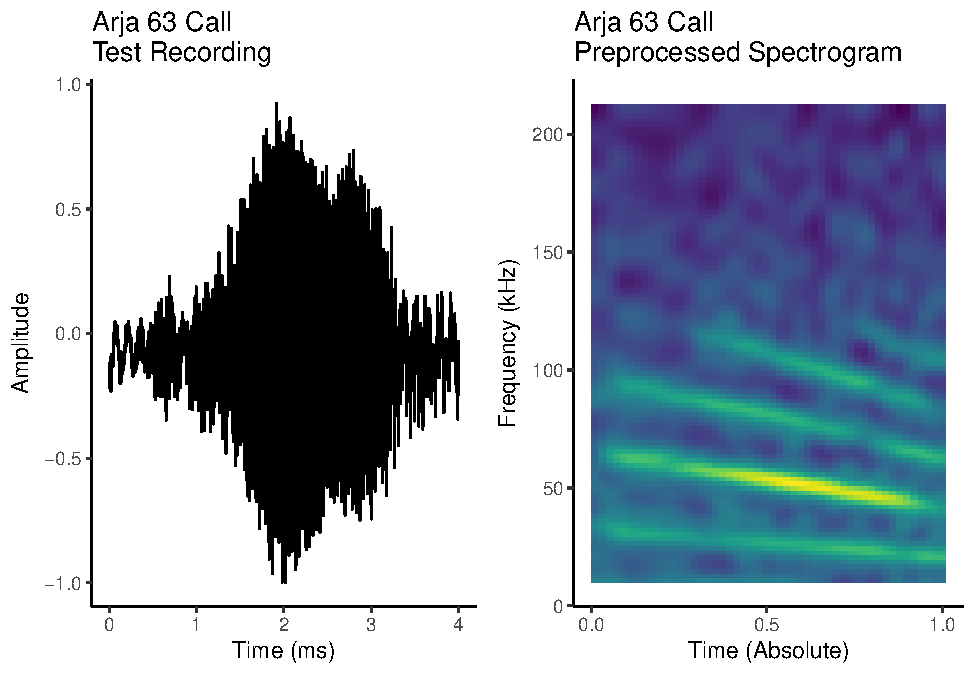
\includegraphics{for_mark_files/figure-latex/recording figure-1.pdf}
\caption{A randomly selected bat call from the species Arja alongside it's corresponding call surface. The call surface is obtained by taking the call spectrogram and treating it as a functional data object. The spectrogram is first smoothed by a robust 2-D spline smoother, then mapped to an absolute time scale and registered in time by a pairwise surface synchronisation, and finally restricted to the 9 - 212 kHz frequency spectrum.}
\label{fig:data}
\end{figure}

Along with this dataset we are given a phylogeny defining the evolutionary relationships between the species of bat. The phylogeny was transcribed from a Bat super-tree published by Collen \cite{collen2012evolution}.

\begin{figure}[htbp]
\centering
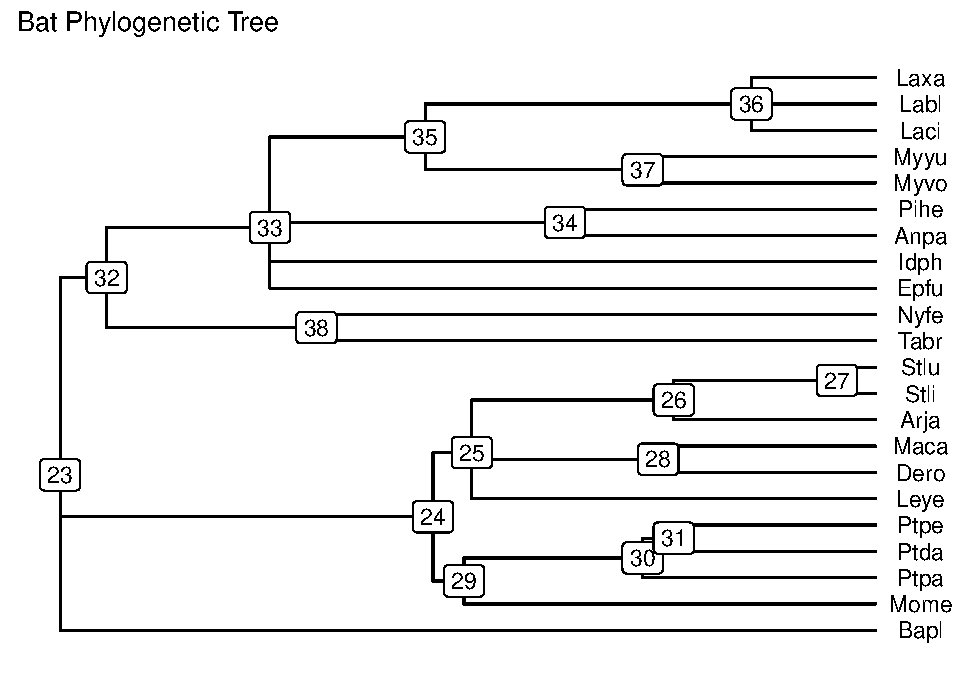
\includegraphics{for_mark_files/figure-latex/phylogeny figure-1.pdf}
\caption{Tree of assumed evolutionary relationships between Bat Species. This phylogeny was transcribed from a recent bat super tree and should represent a `best guess' for the evolutionary relationships between bat species based on the fossil record alongside morphological and molecular studies of evolutionary relationships.}
\label{fig:phylo}
\end{figure}

Implementing the model for evolutionary inference on function valued traits proposed by Jones \& Moriarty \cite{jones2013evolutionary} and further investigated by Hajipantelis \cite{hadjipantelis2013function} allows for reconstruction of ancestral bat call surfaces. By then adapting the RTISI-LA algorithm for spectrogram inversion \cite{zhu2007real} to these call surfaces, an acoustic signal approximating the corresponding echolocation call is produced.

\begin{figure}[htbp]
\centering
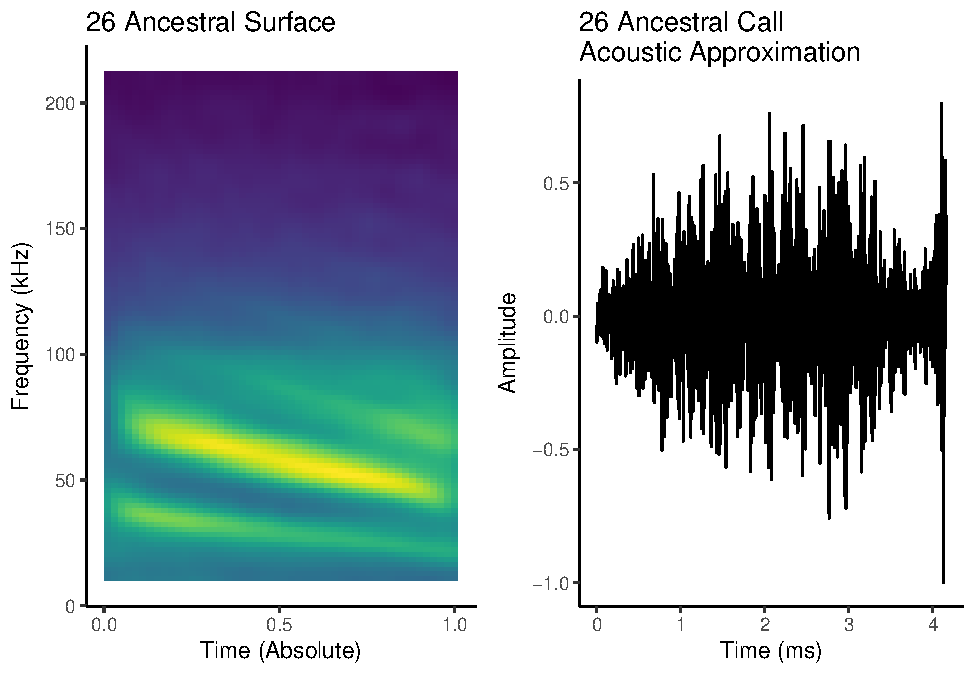
\includegraphics{for_mark_files/figure-latex/ancestral audio-1.pdf}
\caption{Ancestral call surface and acoustic approximation for the common ancestor of Arja, Stli, and Stlu, which corresponds to node 26 in Figure \ref{fig:phylo}. The reconstruction is given by the MAP estimates for the weight of each evolutionary feature at the node. In this case, evolutionary features were identified by a PCA of the smoothed spectrogram surfaces. The acoustic reconstruction was performed assuming a call duration of approximately 4 ms}
\label{fig:ancestral}
\end{figure}

Thus, for a dataset of Mexican Bat echolocation calls and the given phylogeny, reconstruction of ancestral bat echolocation calls has been performed.

\section{The Current Model}

An illustration of the current iteration of a model for the evolution of bat echolocation calls is presented in Figure \ref{fig:current}.

\tikzstyle{rv} = [circle, draw] 
\tikzstyle{plate} = [node distance = 1.25cm]

In the graphical models presented, a \tikz \draw (0, 0) circle (0.1); node represents a random variable, a \tikz \filldraw[fill = gray!50] (0, 0) circle (0.1); represents a random variable for which there are observations, and a \textbullet represents a deterministic parameter in the model. The plates \tikz \draw[rounded corners] (0, 0) rectangle (0.6, 0.3); indicate how many observations / random variables / parameters of each kind there are.

\begin{figure}[htbp]
\centering
\begin{tikzpicture}[node distance = 2cm]
\node[rv, fill = gray!50, label = above left:$y_n$] (y) {};
\node[rv, fill = gray!50, label = above left:$S_n$, right of = y] (S) {}
edge[<-]  (y);

\node[rv, fill = gray!50, right of=S, label = above left:$w_{nq}$] (w) {}
edge[<-] (S);

\node[plate, above right of = w] (ntop) {};
\node[plate, below left of = y, label = 5:$N$] (nbot) {};
\draw[rounded corners] (ntop) rectangle (nbot) ;


\node[right of = w, label = above left:$\hat{w}_q$, rv] (hatw) {};
\node[above of = hatw, label = above left:$\theta_q$] (theta) {\textbullet}
edge [->] (hatw)
edge [<-] (w);
\node[right of = hatw, label = above right:$\mathcal{P}$] (P) {\textbullet}
edge [->] (hatw)
edge [->] (theta);
\node[below of = w, label = above right:$\phi_q$] (phi) {\textbullet}
edge [<-] (S)
edge [->] (w);

\node[plate, above right of = theta] (qtop) {};
\node[plate, below left of = phi, label = 5:$Q$, ] (qbot) {};
\draw[rounded corners] (qtop) rectangle (qbot);

\node[rv, below of=P, label = below left:$\hat{S}$] (hatS) {}
edge[<-] (hatw)
edge[<-] (phi);
\node[right of=hatS, label = below left:$\hat{y}$] (haty) {\textbullet}
edge[<-] (hatS);
\end{tikzpicture}
\caption{A Graphical model detailing the structure of the model for evolution used to produce reconstructions of ancestral bat echolocation calls. Let \(y_n\) be a random variable representing an echolocation call recording. \(S_n\) is the random variable representing the smoothed spectrogram surface given by \(y_n\). The Mexican bat call dataset provides \(N = 1816\) observations of these random variables. The process of transforming a call recording into a spectrogram surface was covered in my 9 month report. The model assumes that each \(S_n\) can be modelled by \(Q\) independent deterministic 'evolutionary features' denoted \(\phi_q\). In this case \(\phi_q\) is inferred by a Principal Components Analysis of \(\{S_n\}_{n = 1}^N\). The weight of each evolutionary feature in \(S_n\) is itself a random variable, where \(w_{nq}\) denotes the weight of \(\phi_q\) in \(S_n\). \(w_{nq}\) is assumed to behave as an Ornstein-Uhlenbeck Gaussian process for which the input space is the phylogeny \(\mathcal{P}\). Each Gaussian process is defined by the deterministic hyperparameters \(\theta_q = [\gamma_q, \ell_q, \sigma_q]^\mathsf{T}\) which are inferred from the data by Type II maximum likelihood estimation over the observed weights. The phylogeny \(\mathcal{P}\) is also assumed to be deterministic in this model and is shown in Figure 2. Ancestral reconstruction is performed by making a prediction for the feature weights, denoted \(\hat{w}\), at some point on \(\mathcal{P}\). Applying these weights to the evolutionary features produces the ancestral call surface which in turn provides an estimate for the ancestral call.}
\label{fig:current}
\end{figure}

Figure \ref{fig:current} illustrates the implementation of the model described in the above introduction, from which reconstructions of ancestral echolocation call surfaces can be produced. This representation describes the model for call spectral density curves presented at the Statistical Data Science conference, the conference paper presented alongside this progress update \cite{meagher2017pgp}, and the current iteration of the model where call spectral density curves have been replaced by call surfaces.

Consider the model than presented in the introduction above with reference to Figure \ref{fig:current}. In order to transform the data \(\{y_n\}_{n=1}^{N}\) into \(\{S_n\}_{n = 1}^N\) some modelling decisions must be made. To find the spectrogram for each call an appropriate window and step size must be chosen. This will affect the time and frequency resolution of the spectrogram. In this case, window size was set to 512 and the step size to 8. The spectrogram is then restricted to the 9 - 212 kHz frequency spectrum as this is the frequency band used by bats for echolocation. The next step involves applying Garcia's robust weighted spline smoothing algorithm \cite{garcia2010robust} to the spectrograms. The algorithm was weighted to ensure that those areas on the spectrogram with the greatest magnitude, corresponding to call harmonics, were not smoothed away in order to reduce noise in unimportant parts of the spectrogram. After smoothing, spectrograms are mapped to an absolute time scale and the grid over which the surface is observed is regularised. In this case, a \(50 \times 104\) grid over \(T \times F\) was used, where \(T \in [0,1]\) and \(F \in  [9, 212]\). With this smoothing and regularisation done, time registration of the call surfaces was performed by adapting pairwise curve synchronisation \cite{tang2008pairwise} to surfaces using a dynamic time warping kernel \cite{damoulas2010bayesian}. In this way \(\{y_n\}_{n=1}^{N}\) was transformed into a new set of observations, \(\{S_n\}_{n = 1}^N\). Further detail on the preprocessing steps described here was included in my 9 month report and can also be found in \cite{pigoli2015analysis}.

The set of call surfaces \(\{S_n\}_{n = 1}^N\) can be considered to be a set of function-valued traits \cite{meyer2005up} each observed at a point \(\mathbf{p}\) in the phylogeny \(\mathcal{P}\) shown in Figure \ref{fig:phylo}, which is assumed to be a deterministic description of the evolutionary relationships between bat species. Thus \(\mathbf{p} \in \mathcal{P}\) can be thought of as a particular species of bat. Jones \& Moriarty \cite{jones2013evolutionary} present results which extend Gaussian processes \cite{rasmussen2006gaussian} for evolutionary inference over phylogenies, referred to as phylogenetic Gaussian processes (PGP). Details on PGPs were included in both my 15 month report and in the accompanying conference paper \cite{meagher2017pgp}. The implementation of the PGP for echolocation call surfaces follows the simulation study performed by Hajipantelis \cite{hadjipantelis2013function} closely. Firstly, 'evolutionary features' must be defined. These can be thought of as deterministic components, a linear combination of which specifies the call surface exactly. Here, a set of Q evolutionary features were defined by a Principal Components Analysis of \(\{S_n\}_{n = 1}^N\), denoted \(\{\phi_q\}_{q = 1}^Q\). For this analysis \(Q = 15\). Secondly, once the set of evolutionary features has been defined, the weight of the \(q^{th}\) component in the \(n^{th}\) call surface, \(w_{nq}\), can be calculated. Finally, it is assumed that \(\{w_{nq}\}_{n = 1}^N\) comes from a zero-mean phylogenetic Ornstein-Uhlenbeck process (POUP) over the input space \(\mathcal{P}\) and is independent of \(\{w_{nq'}\}_{n = 1}^N\) for any \(q' \ne q\). The hyperparameters for the POUP are treated as deterministic parameters and are calculated by type II maximum likelihood estimation given \(\{w_{nq}\}_{n = 1}^N\). The key aspect of the POUP of the \(q^{th}\) evolutionary feature is the kernel defining the covariance matrix,

\begin{equation}
k_q(\mathbf{p}, \mathbf{p}') = \gamma_q \exp\left(\frac{\mathbf{d}(\mathbf{p}, \mathbf{p}')}{\ell_q}\right) + \sigma_q\delta_{\mathbf{p}, \mathbf{p}'},
\label{eq:kernel}
\end{equation}

where \(\gamma_q\) is the phylogenetic noise, \(\ell_q\) is the characteristic length-scale, \(\sigma_q\) is the non-phylogenetic noise, \(\mathbf{d}(\mathbf{p}, \mathbf{p}')\) is the distance between \(\mathbf{p}\) and \(\mathbf{p}'\) in \(\mathcal{P}\), and \(\delta_{\mathbf{p}, \mathbf{p}'}\) is the Kronecker delta. We then let \(\theta_q = [\gamma_q, \ell_q, \sigma_q]^\mathsf{T}\).

Now, having defined the POUP hyperparameters \(\{\theta_q\}_{q = 1}^Q\), and assuming \(\mathcal{P}\), a Gaussian predictive distribution can be found for each of the random variables \(\{\hat{w}_q\}_{q = 1}^Q\) observed at some point \(\hat{\mathbf{p}} \in \mathcal{P}\). Taking the maximum a posteriori (MAP) estimate for \(\{\hat{w}_q\}_{q = 1}^Q\) and denoting this as \(\{\tilde{w}_q\}_{q = 1}^Q\), A reconstruction of the call surface at \(\hat{\mathbf{p}}\) is given by

\begin{equation}
\hat{S} = \sum_{q = 1}^{Q} \tilde{w}_q \phi_q
\label{eq:reconstruction}
\end{equation}

Which in turn provides an estimate of the acoustic call signal at \(\hat{\mathbf{p}}\), \(\hat{y}\).

\section{Developing the Current Model}

The model presented above allows the reconstruction of ancestral bat echolocation call surfaces, which in turn allows the reconstruction of echolocation call acoustic signals. For my collaborators at the Centre for Biodiversity and Environment Research at UCL, this represents a significant step forward in the study of echolocation in bats. It is expected that over the coming months I will be granted access to the EchoBank database of bat call recordings from over 600 species, and that applying this model will result in an impactful publication. However, there remains much work to do.

The first limitation of the model to be addressed is the assumption that \(S_n = \sum_{q = 1}^{Q} w_{nq} \phi_q\). That is to say that the model does not allow for observation noise on the call surface. This in turn means that the likelihood of the observed surfaces, \(p(\mathbf{S} | \Phi, \Theta, \mathcal{P}, \dots)\), for a given model cannot be calculated. Addressing this issue would represent an extension to the methods presented by Jones \& Moriarty \cite{jones2013evolutionary} and Hajipantelis \cite{hadjipantelis2013function}. With a joint likelihood for the call surfaces in place, issues of model selection can be addressed, particularly for comparing models with evolutionary features identified by PCA against features identified by Independent Components Analysis or VARIMAX, for example.

\begin{figure}[htbp]
\centering
\begin{tikzpicture}[node distance = 2cm]
\node[rv, fill = gray!50, label = above left:$y_n$] (y) {};
\node[rv, fill = gray!50, label = above left:$S_n$, right of = y] (S) {}
edge[->]  (y);

\node[rv, right of=S, label = above right:$w_{q}$] (w) {}
edge[->] (S);

\node[plate, above right of = S] (ntop) {};
\node[plate, below left of = y, label = 5:$N$] (nbot) {};
\draw[rounded corners] (ntop) rectangle (nbot) ;

\node[above of = w, label = above right:$\theta_q$] (theta) {\textbullet}
edge [->] (w);
\node[right of = w, label = above right:$\mathcal{P}$] (P) {\textbullet}
edge [->] (w);
\node[below of = w, label = above right:$\phi_q$] (phi) {\textbullet}
edge [->] (S);

\node[plate, above right of = theta] (qtop) {};
\node[plate, below left of = phi, label = 5:$Q$, ] (qbot) {};
\draw[rounded corners] (qtop) rectangle (qbot);

\node[rv, below of=S, label = below left:$\hat{S}$] (hatS) {}
edge[<-] (w)
edge[<-] (phi);
\node[below of=y, label = below left:$\hat{y}$] (haty) {\textbullet}
edge[<-] (hatS);

\node[above of = S, label = above left:$\Sigma$] (phi) {\textbullet}
edge [->] (S);
\end{tikzpicture}
\caption{A proposed extension to the model for the evolution a bat echolocation calls presented in Figure \ref{fig:current}. This model includes a noise process over the call surface, which would allow the calculation of the model evidence. This in turn would facilitate model selection for various sets of evolutionary features, phylogenies, and Ornstein-Uhlenbeck process hyperparameters.}
\label{fig:joint}
\end{figure}

\section{Further Development}

In almost every respect, the model presented in Figure \ref{fig:joint} can be refined further.

Consider \(\mathcal{P}\), the evolutionary relationships between bat species, which has been treated as a deterministic input space in this model. In fact, the true phylogeny is unknown, and so treating \(\mathcal{P}\) as a random variable in the model would be a more accurate representation of our understanding of the problem. 

The same argument applies to the evolutionary features identified, \(\{\phi_q\}_{q = 1}^{Q}\). As such, a probabilistic PCA \cite{tipping1999probabilistic} approach to identifying evolutionary features may be more informative.

The above model assumes that evolution follows an POUP, a popular model for the evolution of continuous character traits introduced by Lande \cite{lande1976natural} and particularly useful for modelling stabilising selection \cite{hansen1997stabilizing}. However empirical analysis of continuous characteristics suggest that models based on stable distributions may be more appropriate \cite{elliot2014inferring} as the heavier tails of these distributions (as compared to a Gaussian distributions) allow for discontinuous jumps in the value of the characteristic between species. One potentially interesting  avenue to explore would be replacing the Gaussian processes in the model with Student-t processes \cite{shah2014student}, which may go some way to accomodating these heavier tails.

It is also fair to say that a 2-D surface may not be the best approach to the Time-Frequency representation of acoustic signals. It is possible that an alternative representation to the call surfaces, such as that proposed by DiCecco \& Gaudette \cite{dicecco2013multi}, may provide a more revealing perspective on the call structure.

While interesting, I do not necessarily feel that any of these any of these aspects of the model are the most important to address. I am of the opinion that relaxing the assumption of independence between the \(Q\) PGPs is the most important next step. An approach to this would be to implement a Gaussian Process Latent Variable Model (GPLVM) \cite{li2016review} \cite{krauth2016autogp}. A GPLVM)may even allow the incorporation of other call characteristics into the model, such as duration, maximum frequency, etc. These call characteristics have been the basis of previous attempts at ancestral reconstruction of echolocation calls \cite{collen2012evolution} and incorporating them may lend more weight to any results.


\section{Thesis Outline}

As part of this report I am including a brief thesis outline. I envision my thesis consisting of four chapters along with an introduction and a conclusion.

In the first chapter I intend to present an ancestral reconstruction of bat echolocation call spectral density curves based on the model presented in Figure \ref{fig:current}, along the lines of the accompanying conference paper \cite{meagher2017pgp}.

In the second chapter I intend to present a joint model for the evolution of echolocation call surfaces, similar to the model presented in Figure \ref{fig:joint}.

The third chapter of my thesis will be based around implementing a LVGPM to relax independence assumption between evolutionary features.

I am uncertain as to the contents of my final chapter, however, I have outlined potential avenues to explore above and expect the most promising of these to become apparent over the coming months. 


\bibliographystyle{plain}
\bibliography{bibliography}

\end{document}
